\subsubsection{Обзор}

В рамках данного исследования была разработана архитектура предиктивной системы нового поколения.
Основное внимание в настоящей работе уделено созданию системы тематического моделирования и аналитического
интерфейса для финансовой предметной области. Логичным продолжением станет построение интерпретируемой
и эффективной модели прогнозирования на основе тематической тональности финансовых публикаций
(новостных статей, пресс‑релизов, постов, транскриптов и др.). Таким образом, настоящая работа
не только демонстрирует принципы функционирования базового модуля, но и формулирует видение того,
каким образом можно расширить её возможностями предсказания цен активов.

Предложенная архитектура опирается на доказавшие свою надёжность подходы смешанного прогнозирования ---
сочетание сверточных и рекуррентных нейронных сетей (CNN-LSTM) \parencite{Hochreiter1997LSTM, CNN1998lecun, CNN_LSTM2020finance}.
Это решение позволяет одновременно учитывать глобальные долгосрочные тенденции (например, общий тренд рынка)
и локальные краткосрочные паттерны (такие как «голова и плечи», «двойное дно» и другие структуры,
обусловленные поведенческой экономикой).

При этом важно помнить о разнообразии исходных данных. Для прогнозирования обычно используют биржевые метрики
(OHLCV и т.п.) и производные технические индикаторы (RSI, MACD и др.).
В нашем исследовании к ним добавляются текстовые данные как внебиржевой источник. В дальнейшем в
качестве дополнительных модальностей могут быть привлечены графовые представления связей, изображения,
аудио‑ и видеозаписи. Таким образом, на текущем этапе мы работаем с тремя модальностями, каждая из которых
несёт самостоятельную смысловую нагрузку и способна объяснить динамику цен независимо, но их взаимодействие
может как усиливать полезный сигнал, так и вносить шум.

В данном исследовании архитектура была построена на основе CNN-LSTM с использованием медленного слияния.
Основной инженерный вызов состоял в согласовании пространственно‑временных форм признаков разных модальностей.
Для решения этой задачи в архитектуру введён Механизм Кэширования Признаков (Feature Caching Mechanism, FCM),
который синхронизирует тональностные векторы текстовой модальности с биржевыми временными рядами.

Дополнительно текстовая ветвь подвергается предобработке: на основе разработанной системы тематического
моделирования вычисляются тематические тональности публикаций. Это позволяет получить специализированные
оценки по каждой теме, что даёт преимущество перед использованием единой общей тональности.


\begin{figure}[H]
    \centering
    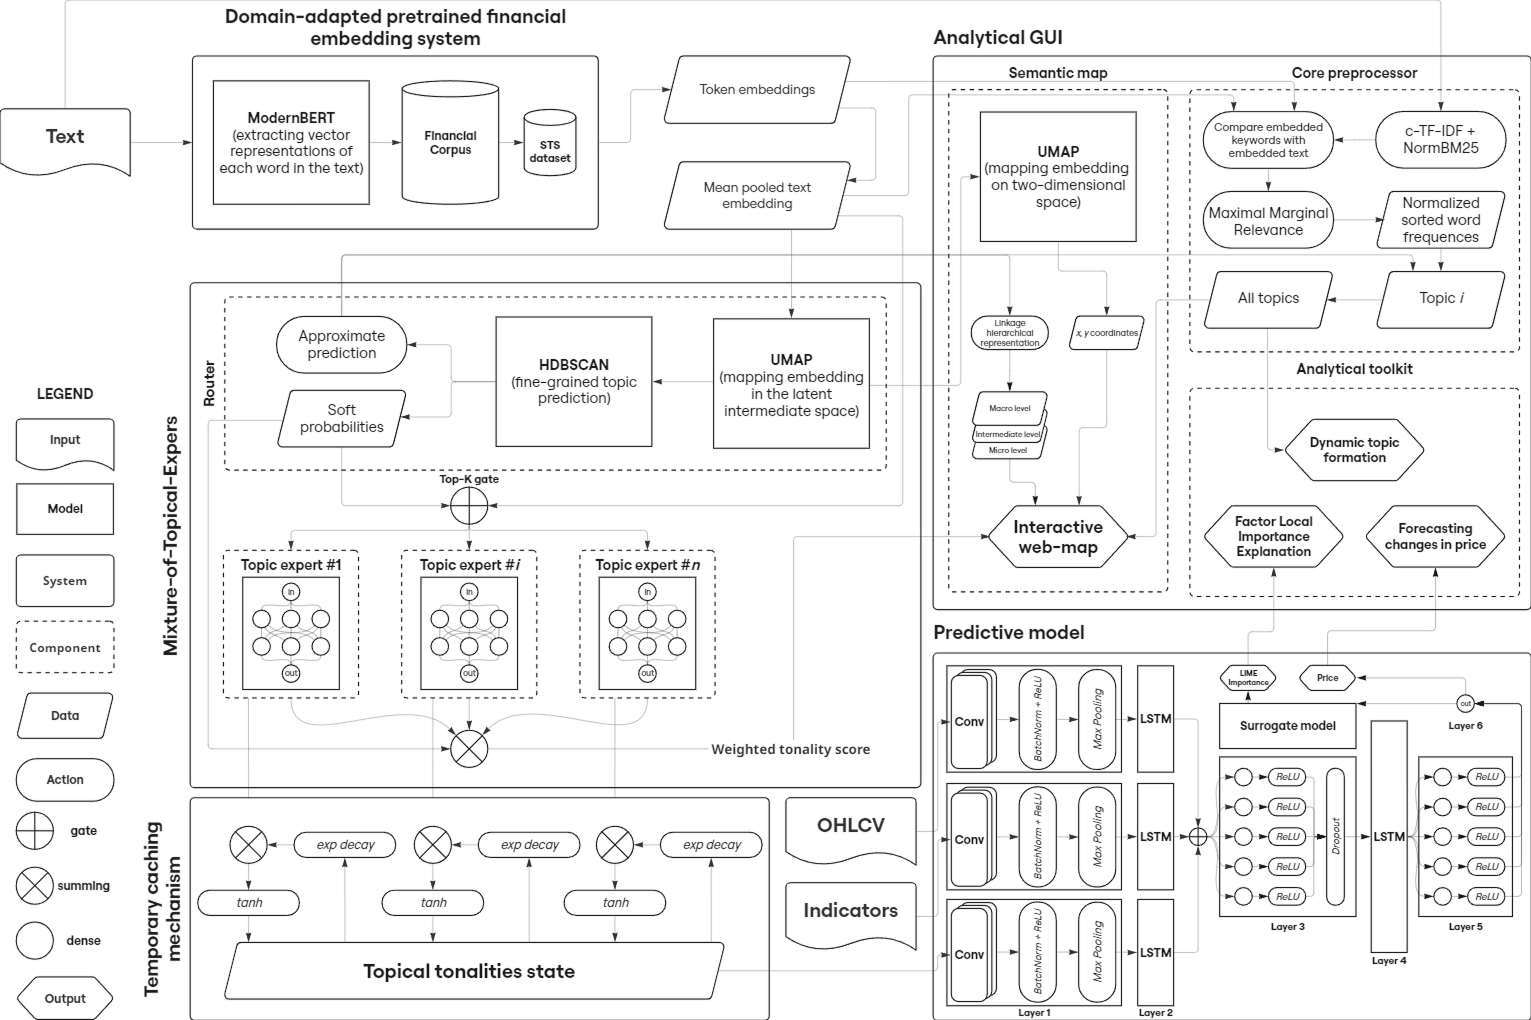
\includegraphics[width=1\linewidth]{img/architecture_overview.png}
    \caption{Обзор спроектированной архитектуры FinABYSS.}
    \label{fig:architecture_overview}
\end{figure}

Спроектированная система состоит из пяти основных модулей (Изображение \ref{fig:architecture_overview}):

\begin{itemize}
    \item Финансовая языковая модель (доменно-адаптированная, тонко настроенная для задачи STS), выдающая векторные представления текста целиком и для каждого токена.
    \item Смесь тематических экспертов (Mixture-of-Topical-Experts, MoTE), формирующая тональность публикации по каждой теме.
    \item TCM, выравнивающий тематические векторы по временным меткам биржевых данных.
    \item Ядровая предиктивная модель с CNN-LSTM и медленным слиянием, обрабатывающая все модальности и предсказывающая цену актива.
    \item Аналитический графический интерфейс (GUI), агрегирующий промежуточные результаты для последующего финансового анализа.
\end{itemize}

Таким образом, созданная архитектура представляет собой мощный и адаптируемый инструмент
для прогнозирования стоимости финансовых активов на основе комплексной оценки тематических сентиментов публикаций.

\subsubsection{Эмбеддинговая система}
Приступая к рассмотрению отдельных блоков разработанной архитектуры, следует начать с этапа предобработки данных.
Наиболее ресурсоёмким и сложным из них является подготовка внебиржевых текстовых источников.

Сразу после поступления в систему текст проходит первичную обработку с помощью доменно‑адаптированной финансовой
эмбеддинговой модели, настроенной на задачу STS. В результате работы этой
модели извлекаются векторные представления для каждого токена, что позволяет сохранить тонкие контекстные связи
внутри предложений. По мере появления новых версий эмбеддинговых моделей важно регулярно обновлять базовую модель
и повторно адаптировать её к специфике финансового домена.

Простейший путь доменной адаптации включает дополнительную стадию обучения на задаче MLM. В качестве корпуса
для этой цели может использоваться корпус финансовых публикаций, сформированный в ходе настоящего исследования,
либо его расширенная версия, а также другие релевантные текстовые корпусы. Для тонкой настройки под задачу STS
иногда применяют небольшие размеченные датасеты, однако для экономии ресурсов возможно обойтись и без них,
используя методы контрастивного обучения на случайных подвыборках основного корпуса \parencite{gao2021simcse}.

После извлечения эмбеддингов токенов производится их агрегирование: обычно применяется усреднение, что даёт векторное
представление всего документа. Далее документ и его эмбеддинги (как токенов, так и усреднённый вектор) передаются
в аналитический модуль для визуализации и интерпретации результатов. Параллельно вектор документа направляется
в блок MoTE, где на его основе формируются тематические тональности публикации.

В качестве конкретной реализации в данном исследовании используется модель 'gte-modernbert-base', построенная на архитектуре
ModernBERT. Несмотря на то, что изначально она не проходила доменную адаптацию, она демонстрирует высокую эффективность:
при кластеризации эмбеддингов удалось получить DBCV-индекс 0.407, а визуальный и контекстуальный анализ показали чёткое разделение тематических групп.

Таким образом, предложенный этап предобработки обеспечивает:

\begin{itemize}
    \item Сохранение глубоких семантических связей на уровне токенов и всего документа.
    \item Гибкость и воспроизводимость процесса адаптации модели к финансовому корпусу.
    \item Интеграцию результатов в соседние блоки архитектуры --- MoTE и аналитический GUI.
\end{itemize}

\subsubsection{Смесь тематических экспертов}

Данный блок использует современную архитектуру Mixture-of-Experts (MoE), успешно применяемую в крупных
языковых моделях (например, Mixtral 8×7B, DeepSeek R1) и в исследованиях Google (Switch Transformer) \parencite{fedus2022switch}.
Основные компоненты данного блока --- обучаемый роутер и множество экспертов --- позволяют динамически активировать
лишь небольшую часть параметров при инференсе, обеспечивая высокую пропускную способность и эффективность
\parencite{shazeer2017outrageously}. Специально для анализа финансовых текстов эксперты тематически
специализированы, что повышает интерпретируемость и точность оценки тональности публикаций.

Архитектура MoE построена на принципе условных вычислений: лишь часть подсетей («экспертов») активна
для каждого входного примера, что снижает вычислительные затраты при огромном общем числе параметров
\parencite{shazeer2017outrageously}.


\begin{itemize}
    \item Роутер получает на вход эмбеддинг документа и вычисляет распределение «весов» для всех экспертов,
    после чего выбирает либо топ-K экспертов, либо тех, чей вес превышает заданный порог, являющийся гиперпараметром.
    \parencite{fedus2022switch}.
    \item Эксперты представляют собой неглубокие feed-forward сети, каждая из которых специализируется на своей
    тематике (в контексте работы --- на одной из финансовых тем) \parencite{shazeer2017outrageously}.
\end{itemize}

При обработке каждого эмбеддинга активизируется лишь малая часть экспертов --- обычно по Top $K$
(выбор $K$ наиболее релевантных экспертов) или по пороговому значению (вес эксперта выше заданного порога) ---
что делает MoE чрезвычайно экономным с точки зрения вычислений при колоссальном общем числе параметров \parencite{fedus2022switch}.
Значения $K$ и $\theta$ выступают гиперпараметрами и настраиваются на валидационных данных.

Для анализа финансовых текстов MoE-модель является логичным выбором, поскольку публикации часто содержат смесь
смежных тематик (макроэкономика, корпоративные отчёты, геополитика и др.), и требуется оценить тональность
под разными углами. Эксперты позволяют формировать специализированные оценки по каждой теме одновременно,
сохраняя «чистоту» низкоуровневой обработки и обеспечивая интерпретируемость результатов \parencite{jacobs1991adaptive}.
Тем не менее, стоит отметить и высокую сложность подбора $K$ или $\theta$ гиперпараметров \parencite{jacobs1991adaptive}.

Вместо обучения экспертов на субъективно размеченных данных их параметры оптимизируются обратным распространением ошибки,
поступающей из блока предсказания цен активов. Это гарантирует, что каждый эксперт обучается напрямую на влиянии публикаций
на стоимость активов, а не на внешних аннотациях \parencite{shazeer2017outrageously}. После получения тематических тональностей
они агрегируются взвешенным суммированием с учётом вероятностей тем, нормализуются и направляются в аналитическую
систему для визуализации, а также в механизм кэширования признаков для синхронизации с биржевыми данными.

Таким образом, блок MoTE на базе MoE обеспечивает обеспечивает сочетание масштабируемости,
эффективности и интерпретируемости при анализе финансовых текстов. Динамическая активация небольшого числа
экспертов позволяет обрабатывать огромные модели без пропорционального роста вычислений, а обучение экспертов через
сигнал от модели прогнозирования цен делает оценку тональностей объективной и близкой к экономической реальности.
Таким образом, предлагаемая архитектура открывает новые возможности для точного прогнозирования и глубокого анализа
влияния текстовых публикаций на стоимость финансовых активов.

\subsubsection{Механизм кэширования признаков}
FCM представляет собой центральный компонент архитектуры, обеспечивающий синхронность между биржевыми данными
(регулярно поступающими временными рядами) и внебиржевыми текстовыми «тиками», разбросанными во времени.
Когда из блока Смеси Тематических Экспертов поступает новая оценка тональности публикации по теме $i$,
она моментально добавляется в матрицу накопительных экспоненциально сглаженных значений по Формуле \ref{eq:exp_decay}:

\begin{equation}\label{eq:exp_decay}
    x_{i,t}=x_{i, t-1} + x_{i, 0} \cdot e^{-\lambda \cdot t},
\end{equation}

где $x_{i, 0}$ --- исходная тональность по теме $i$, $x_{i,t-1}$ --- предыдущее сглаженное значение,
а $\lambda$ --- гиперпараметр скорости экспоненциального «затухания» сигнала. Такой подход отражает
запаздывающую и сглаженную во времени реакцию участников рынка на публикации.

Данный подход учитывает, что реакция участников рынка на информационные события задерживается и распределена
во времени: первая «волна» восприятия быстро затухает, за ней следуют более плавные и длительные эффекты,
что в финансах традиционно моделируется экспоненциальным спадом.

Так как исходные тональности нормированы в диапазоне $[-1,1]$, накопительное суммирование по первой формуле
может выходить за эти границы. Чтобы сохранить скалирование в допустимых интервалах и придать плавность
накоплению, предлагается повторно нормировать результаты с помощью гиперболического тангенса (Формула \ref{eq:tanh1}):

\begin{equation}\label{eq:tanh1}
    tone_{i, t} = \tanh(tone_{i, t-1} + x_{i,t}) =
    \cfrac{
        \tanh{(tone_{i, t-1})} + \tanh{(x_{i,t})}
    }{
        1 + \tanh{(tone_{i, t-1})} \cdot \tanh{(x_{i,t})}
    }.
\end{equation}

что эквивалентно Формуле \ref{eq:tanh2}:

\begin{equation}\label{eq:tanh2}
    tone_{i, t} =
    \cfrac{
        (1-e^{-2 \cdot tone_{i, t}})+(1-e^{-2x_{i,t}} - (1-e^{-2 \cdot tone_{i, t}}) \cdot(1-e^{-2x_{i,t}})
    }{
        (1+e^{-2 \cdot tone_{i, t}})+(1+e^{-2x_{i,t}} - (1+e^{-2 \cdot tone_{i, t}}) \cdot(1+e^{-2x_{i,t}})
    },
\end{equation}

где $tone_{i, t}$ --- текущая нормированная экспоненциально сглаженная тональность по теме $i$ на момент $t$.

В результате непрерывной работы FCM формируется матрица накопительных тематических тональностей,
обновляемая при каждом поступлении текстового «тика». Пока биржевые данные (OHLCV и индикаторы)
отсутствуют, этот временной ряд накапливает сигналы «рыночного сентимента». Как только в систему
приходит новый временной ряд биржевых измерений (с учётом сетевой задержки $\delta$), накопленные
и нормированные тональности конкатенируются с ценовыми и индикаторными данными и передаются
в предиктивную модель для совместной обработки.

Динамический процесс работы механизма проиллюстрирован на Изображении \ref{fig:feature_caching_mechanism}.
Во входной момент кэш инициализируется нулевыми значениями, затем при каждом поступлении текстовой оценки
обновляется по формуле \ref{eq:exp_decay}, после чего нормируется функцией гиперболической тангенсоиды. По достижении триггера ---
момента $t$ или поступления биржевых данных в момент $t+\delta$ --- объединённый временной ряд передаётся дальше.

\begin{figure}[H]
    \centering
    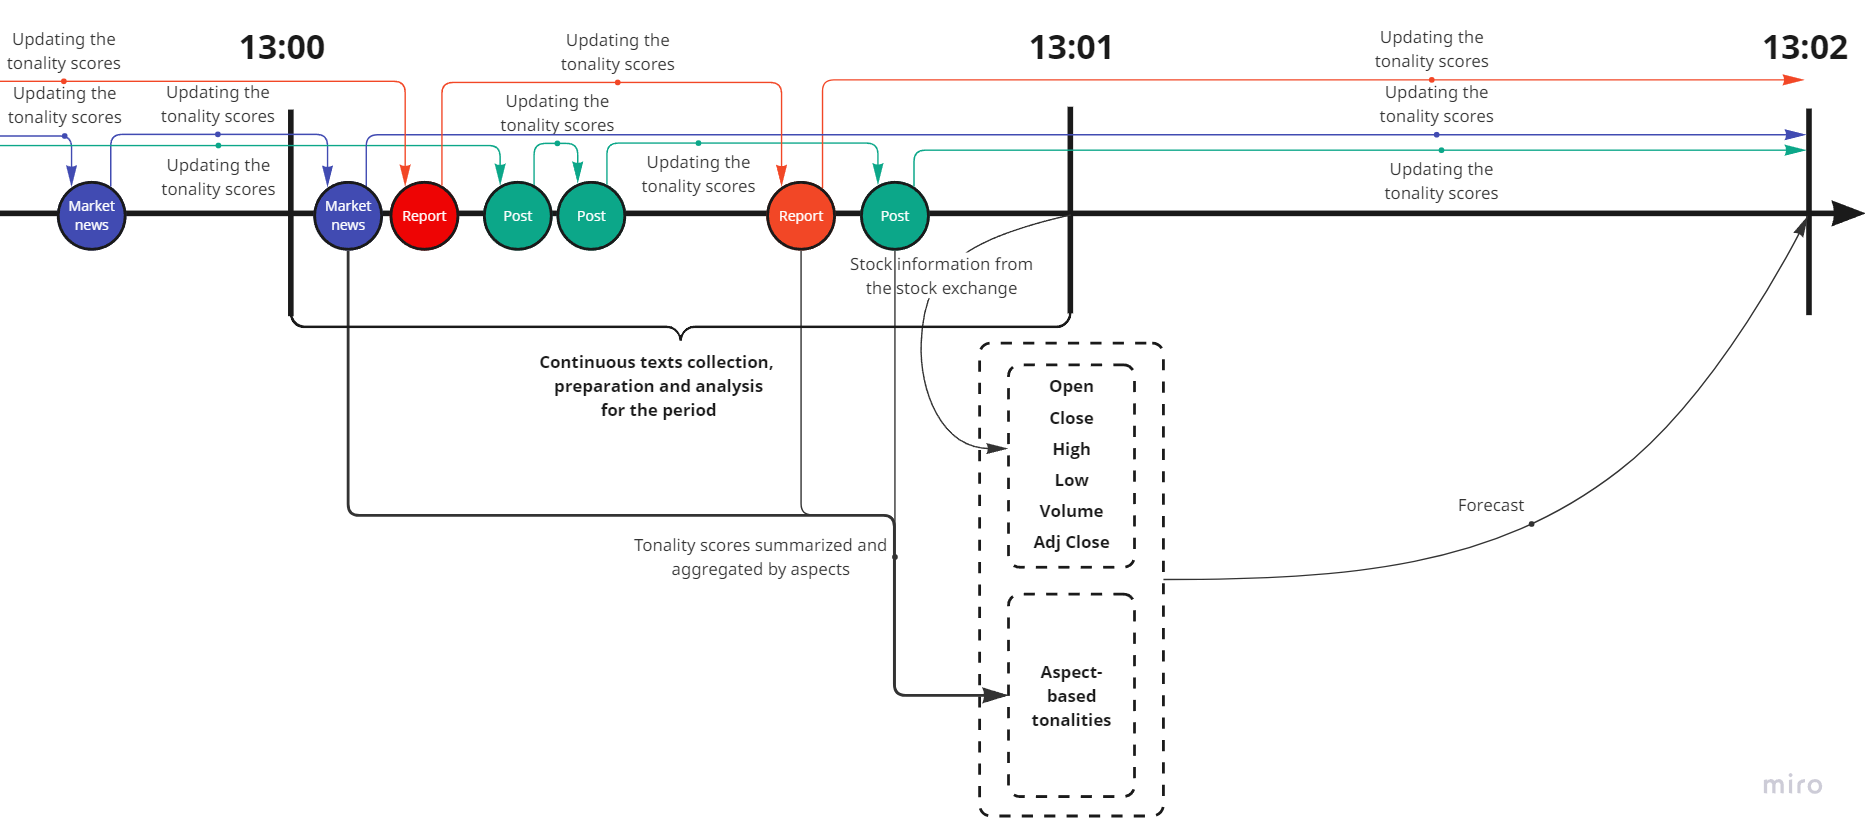
\includegraphics[width=1\linewidth]{img/feature_caching_mechanism.png}
    \caption{Динамическая репрезентация сихронизации внебиржевых данных при помощи FCM на минутном свечевом интервале.}
    \label{fig:feature_caching_mechanism}
\end{figure}

Таким образом, FCM выполняет следующие функции: преобразует нерегулярные текстовые
события в непрерывный многомерный временной ряд, применяет адекватное финансовым реалиям сглаживание и масштабирование
тональностей, а также гарантирует синхронизацию с биржевыми данными. Это обеспечивает согласованность и стабильность
входных признаков в предиктивной модели и способствует повышению точности прогнозирования стоимости финансовых активов.

\subsubsection{Предиктивная модель}
В предлагаемой гибридной архитектуре мы стремимся объединить преимущества свёрточных слоёв для локального
выделения признаков и рекуррентных модулей для моделирования длительных зависимостей, одновременно
обеспечив адаптивное слияние количественных и качественных сигналов. На вход подаётся многомерный
временной ряд длины $T$, в котором каждому временному шагу $t$ соответствует вектор
$x_t = [x_t^{\rm price}, x_t^{\rm ind}, x_t^{\rm sent}]$, где $x_t^{\rm price}\in\mathbb{R}^{C_p}$
содержит OHLCV, $x_t^{\rm ind}\in\mathbb{R}^{C_i}$, а $x_t^{\rm sent}\in\mathbb{R}^{C_s}$ ---
набор скользящих и сглаженных значений тональностей новостей.

Сначала данные разбиваются на три ветви: «Price», «Indicator» и «Sentiment». Каждая ветвь проходит два
базовых уровня обработки. На первом уровне в каждой ветви последовательность $\{x_t^{(\cdot)}\}_{t=1}^T$
пропускается через одномерную свёртку с небольшими ядрами и операциями пулинга (Формула \ref{eq:relu_pooling})

\begin{equation}\label{eq:relu_pooling}
    y^{(\ell+1)}_{t} = \mathrm{ReLU}\bigl(W^{(\ell)} * y^{(\ell)}_{t} + b^{(\ell)}\bigr), \\
    y^{(\ell+\tfrac12)}_{t} = \max\bigl(y^{(\ell+1)}{t},\,y^{(\ell+1)}_{t+1}\bigr).
\end{equation}

где символ $*$ обозначает свёртку по времени, функция активации $\mathrm{ReLU}$ определяется следующим образом (Формула \ref{eq:relu}):

\begin{equation}\label{eq:relu}
    \mathrm{ReLU}(x)=\max(0, x).
\end{equation}

Затем операция max пулинга сокращает временную размерность вдвое. Такая последовательность позволяет
в начальных слоях выделить локальные шаблоны внутри каждого потока, будь то короткие ценовые колебания,
импульсы индикаторов или флуктуации сентимента.

Далее на выходе пулинга в каждой ветви обучается рекуррентный модуль LSTM, который моделирует накопление
и забывание информации с учётом длительных временных зависимостей. Пусть $h_t$ и $c_t$ — скрытое состояние
и ячейка памяти LSTM; их эволюция задаётся стандартными уравнениями входных-, забывающих- и выходных-гейтов. Благодаря
этому каждая ветвь самостоятельно учится определять, какие локальные признаки значимы для прогнозирования
на более отдалённых временных горизонтах.

После того как каждая ветвь выдала своё скрытое состояние $h_t^{\mathrm{price}}$, $h_t^{\mathrm{ind}}$, $h_t^{\mathrm{sent}}$
на каждом временном шаге, происходит этап адаптивного слияния. Для этого векторная конкатенация $u_t$ пропускается через
гейтовый слой (Формула \ref{eq:gate})

\begin{equation}\label{eq:gate}
    g_t = \sigma\bigl(W_g\,u_t + b_g\bigr).
\end{equation}

где $\sigma$ --- сигмоида и $g_t\in(0,1)^{\dim u}$ задаёт поэлементные коэффициенты,
контролирующие относительный вклад каждого потока. Само же объединённое представление вычисляется как

\begin{equation}
    m_t = g_t\odot u_t + (1-g_t)\odot\mu(u_t).
\end{equation}

где $\mu(u_t)$ может быть усреднением или другим агрегатором компонентов вектора $u_t$.
Такой механизм позволяет модели динамически переключаться между акцентом на ценовых паттернах,
индикаторных сигналах или сентименте в зависимости от контекста конкретного временного отрезка.

Объединённая последовательность $\{m_t\}_{t=1}^{T/2}$ затем вновь поступает в рекуррентный модуль
LSTM, который, подобно предыдущим, аккумулирует информацию о совместном развитии трёх модальностей
на более высоком уровне абстракции. Его выходом служит последнее скрытое состояние
$h_{T/2}^{\mathrm{merge}}$, содержащее сжатое резюме всей истории. Для придания нелинейности
и дополнительного измерения выразительности это состояние может быть пропущено через полносвязный
слой с функцией $\mathrm{ReLU}$, а затем — через слой Dropout для регуляризации и смягчения переобучения.

Наконец, заключительный слой без активации переводит полученный вектор в одномерное предсказание
$\hat y$, которое интерпретируется как новая цена (в режиме регрессии).

Также, стоит отметить, что, в целях, локальной интерпретируемости оценок тональности важную роль
в архитектуре играет наличие отдельной суррогатной модели, которая на основе выборки ряда
тональностей, полученного из Feature Caching Mechanism, с дополнительными волнениями,
оценивает вклад каждой тематической тональности в итоговое предсказание стоимости актива.

Таким образом, предложенная гибридная архитектура объединяет локальную детекцию паттернов
(одномерной свёртки), способность LSTM моделировать длительные зависимости, а также механизм
адаптивного слияния, позволяющий динамически регулировать вклад ценовых, индикаторных и сентиментальных
сигналов. Это обеспечивает высокую точность прогнозов при умеренной вычислительной сложности
и прозрачности модели относительно используемых признаков, при этом оставаясь более лёгкой
и прозрачной по сравнению с трансформерными аналогами.

\subsubsection{Аналитический графический интерфейс}
\label{sec:gui}
В завершение описания архитектуры FinABYSS необходимо остановиться на ключевом пользовательском компоненте ---
Аналитическом GUI. Этот модуль аккумулирует результаты всех предыдущих этапов:
от предобработки внебиржевых текстов и их тематической интерпретации в блоке MoTE до конкатенации
с ценовыми и индикаторными рядами в предиктивной модели. На вход GUI поступают промежуточные и финальные данные,
а его задача --- привести их в наглядный, интерактивный и аналитически релевантный вид. GUI состоит
из трёх взаимосвязанных компонент, реализующих постобработку данных, предоставление инструментов
глубокого анализа и визуализацию семантических связей между документами.

Первый компонент --- ядровой постпроцессор --- отвечает за трансформацию «сырых» выходов предыдущих
блоков в упорядоченные и компактные репрезентации. На этапе инициализации он вычисляет относительные
частоты терминов с помощью BM25-модификации TF-IDF и дополнительной нормализации, что удаляет шумовые
и часто встречающиеся, но семантически незначимые токены (например, названия агрегаторов типа Zacks).
Далее, после получения эмбеддингов токенов и всего документа из доменно‑адаптированной языковой модели,
выполняется ранжирование $n$‑грамм по частотам с учётом косинусного сходства между векторами токенов
и документного вектора. Для обеспечения баланса между релевантностью и диверсификацией подсистемы
применяется алгоритм MMR: при разбиении на биграммы MMR устраняет дублирующиеся или избыточно близкие
по смыслу фрагменты, оставляя наиболее информативные. Например, из сырых биграмм «ai» и «ai stocks»
в зависимости от относительной частоты и семантической близости могут сохраниться либо «ai» и «stocks»,
либо только «ai stocks», либо только «ai», что повышает однородность итогового словаря и уменьшает
избыточность.

После применения MMR словарь сортируется по итоговым частотам, и постпроцессор получает от блока MoTE метку
кластера, к которому принадлежит текущий документ. На основе этой кластерной принадлежности осуществляется
инкрементальное обновление c‑TF‑IDF статистики: накопленные частоты слов внутри каждого кластера корректируются
с учётом новой публикации, что обеспечивает адаптивность и учёт эволюции тематических трендов во времени
и используется для динамического тематического моделирования. Параллельно от постпроцессора поступают два
потока данных: обогащённые частотные признаки и другие извлечённые метаданные текста направляются
в аналитический инструментарий, а сам очищенный и классифицированный текст с эмбеддингами --- в Семантическую карту.

Второй компонент --- Аналитический инструментарий --- представляет собой набор визуальных и интерактивных элементов,
позволяющих пользователю углублённо исследовать динамику тематических трендов и их влияние на цены активов.
Через дашборды можно получать:

\begin{itemize}
    \item исторические графики тональностей по каждой теме, совмещённые с ценовыми рядами и техническими индикаторами;
    \item динамические корреляционные матрицы между темами и движениями цен;
    \item сводные отчёты по влиянию макро‑, мезо‑ и микротем на волатильность и трендовые движения;
    \item агрегированные показатели рыночной тональности (взвешенная суммарная тональность по всем темам) с трендовыми линиями.
\end{itemize}

Инструментарий разработан с учётом будущего расширения: при добавлении новых модальностей
(изображения, графовые данные, аудио‑ или видеопотоки) к нему легко интегрируются модальностно‑специфичные
виджеты --- например, интерактивные облака ключевых сущностей, графы взаимосвязей эмитентов
или тепловые карты тональностей в голосовых и видео‑форматах.

Третий компонент --- Семантическая карта --- реализует двумерную визуализацию эмбеддингов документов.
На основе заранее обученной модели понижения размерности каждое документное представление из латентного
пространства, где проводилась кластеризация, отображается в координатах $(x,y)$. Параллельно используется
аппроксимальный предсказатель темы из блока Смеси Тематический Экспертов: по каждому документу
определяется иерархически организованная тройка тематических меток --- на макро‑, мезо‑ и микроверсиях.
Цвет, размер и форма маркеров на карте кодируют принадлежность к кластеру, силу тональности и объём
текста. Это позволяет анализировать не только пространственное соседство публикаций, но и их тематическую
многоуровневую структуру, быстро выявлять периферийные и центральные документы, а также отслеживать
эволюцию тематических сообществ.

В совокупности GUI создаёт единую интерактивную панораму, в которой результаты глубочайших вычислительных блоков
--- от FCM и MoTE до гибридной CNN-LSTM предиктивной модели — превращаются в интуитивно понятный и аналитически
ёмкий инструмент. Пользователь получает возможность не просто просматривать прогнозы цен, но и детально исследовать
причинно‑следственные связи между медиасигналом и движением рынка.

Аналитический графический интерфейс FinABYSS обеспечивает сквозную визуализацию и интерпретацию выходных данных
системы, интегрируя частотные, тематические и эмбеддинговые признаки в три взаимосвязанных подсистемы. Ядровой
постпроцессор трансформирует «сырые» текстовые и числовые данные в компактные и репрезентативные признаки,
аналитический инструментарий предлагает гибкие средства глубокого исследования влияния тем на стоимость активов,
а семантическая карта даёт наглядное отображение многомерных эмбеддингов с учётом иерархической тематики.
Благодаря такому сочетанию технологической мощности и удобства взаимодействия GUI выступает завершающим,
но не менее важным звеном в конвейере прогнозирования, обеспечивая прозрачность, адаптивность и наглядность
результатов для экспертов в области финансов.
